\documentclass[12pt]{article}
\usepackage[vmargin=20mm, hmargin=15mm]{geometry} 
\usepackage{multicol}
\usepackage{datetime}
\usepackage{array}
\usepackage{lipsum}
\usepackage{graphicx}
\usepackage{mwe}
\usepackage[square]{natbib}
%\usepackage{url}
%\usepackage{hyperref}
%\usepackage[svgnames]{xcolor}
%\hypersetup{
 % colorlinks,
 % urlcolor=Blue}
  
\geometry{a4paper} 
\frenchspacing
\parindent 0pt
\parskip 6pt
\setlength\columnsep{15pt}

\newcommand{\docvec}{\texttt{doc2vec}}
\newcommand{\wordvec}{\texttt{word2vec}}

%%% BEGIN DOCUMENT
\begin{document}
\centerline{\large NLP Assignment 2 Report}
\vspace{0.1in}
\centerline{\Large\bf Doc2Vec for Sentiment Detection of Reviews}
\vspace{0.1in}
\centerline{\large {\bf{Z\'ebulon Goriely, Queens', zg258}}}
\vspace{0.1in}
%\centerline{\large {\today}}
\centerline{\large{Friday 22\textsuperscript{nd} November, 2019}}
\vspace{0.05in}
\centerline{Word Count: 983\footnote{\emph{texcount docs/assignment2/report.tex}}}
\vspace{0.2in}

\makeatletter
\newenvironment{tablehere}
  {\def\@captype{table}}
  {}

\newenvironment{figurehere}
  {\def\@captype{figure}}
  {}
\makeatother

%%% BEGIN BODY OF TEXT
\begin{multicols}{2}

\section{Introduction}

\citet{le2014distributed} introduced \docvec~for learning embeddings for sequences of words. Here, I investigate the use of \docvec~document vectors in the task of sentiment detection, using a Support Vector Machine (SVM) classifier.

I compare the performance of the classifier trained with \docvec~vectors with the same classifier trained with simple word-frequency and presence-based vectors. Finally, I examine means of qualitatively analysing the hypothesis that \docvec~encodes semantics, in particular how sentiment-coding adjectives are represented.

\section{Background}

To classify reviews, I use an SVM classifier trained and tested on document vectors. I was given a dataset of 1000 positive and 1000 negative movie reviews in the framework of a course in NLP.

\begin{table*}[t]
\centering
 \begin{tabular}{ r l c}
 \bf{Hyperparameter} & \bf{Description} & \bf{Best Value} \\ [0.5ex] 
 \hline
Vector Size &  Dimension of word vectors & 124 \\ 
Window Size & Left/right context window size & 6 \\
Min Count & Minimum frequency threshold for word types & 20 \\
Negative Sample & No. of negative word samples & 0 \\
Epoch & Number of training epochs & 5 \\
\end{tabular}
\caption{A description of \texttt{doc2vec} hyperparameters and the best values found for this task.} \label{table:params}
\end{table*}

\begin{table*}[t]
\centering
 \begin{tabular}{|c|c|c|c|} 
 \hline
  & Unigram-frequency & Unigram-presence & doc2vec \\ [0.5ex] 
 \hline\hline
Unigram-frequency & 1 &  $2.00\times 10^{-4}$ & $2.00\times 10^{-4}$\\
 \hline
Unigram-presence & $2.00\times 10^{-4}$ & 1  & $1.60\times 10^{-3}$\\
 \hline
doc2vec & $2.00\times 10^{-4}$ & $1.60\times 10^{-3}$ & 1 \\
 \hline
\end{tabular}
\caption{The significance of difference between systems from Table \ref{table:accuracies}.} \label{table:p-values}
\end{table*}

\subsection{Support Vector Machine}

\citet{pang2002thumbs} introduced the use of SVM classifiers for sentiment analysis, operating on document vectors.

A frequency-based document vectors is defined $\vec{d} := (n_{1}(d), n_{2}(d),\ldots,n_{m}(d))$ where $n_{i}(d)$ is the occurrences of feature $f_{i}$ in document $d$.

A presence-based document vector is defined as $\vec{d} := (s_{1}(d), s_{2}(d),\ldots,s_{m}(d))$ where
\[
s_{i} =
\left\{
	\begin{array}{ll}
		1  & \mbox{if $d$ contains $f_{i}$} \\
		0 & \mbox{otherwise}
	\end{array}
\right.
\]

Using supervised learning, the procedure produces a hyperplane represented by the vector $\vec{w}$ which divides the vectors into two classes. This hyperplane exists in the n-dimensional vector space of the document vectors.

This allows for classification to proceed by determining which side of the hyperplane each $d_{i}$ falls on.

\subsection{Doc2Vec}

\citet{mikolov2013distributed} introduced the ideas of skipgrams and \wordvec~to create compact vector-space representations of words. Unlike the frequency-based document vectors and presence-based vectors, the dimensions of these vectors are not directly interpretable.

\citet{le2014distributed} extended this idea to \docvec~which learns embeddings of \emph{sequences} of words. A key feature is that it is agnostic to granularity, generating fixed-length vectors from variable-length pieces of text. In this case, I train \docvec~to output document embeddings, a new type of vector that Le and Mikolov claim is effective for sentiment analysis.

The two architectures in \docvec~are the distributed memory and distributed bag of words model which are closely correlated to the \wordvec~ and skip-gram models respectively.

\section{Method}

Selecting unigrams as a feature, I compare the performance of training and testing an SVM classifier on:
\vspace{-\topsep}
\begin{itemize}
\setlength{\parskip}{0pt}
\setlength{\itemsep}{0pt plus 1pt}
	\item frequency-based document vectors
	\item presence-based document vectors
	\item vectors inferred from a trained \docvec~model
\end{itemize}

I implemented\footnote{https://github.com/ZGoriely/cambridge-nlp} the SVM classifier using Joachim's (1999) $SVM^{light}$ package\footnote{http://svmlight.joachims.org}, using default parameters. For the \docvec~implementation, I used the gensim library\footnote{https://radimrehurek.com/gensim}.

I trained the \docvec~model on a large external corpora of 100,000 movie reviews provided by the Stanford Large Movie Review Dataset \citep{maas-EtAl:2011:ACL-HLT2011}. In a 2014 evaluation of \docvec~, \citet{lau2016empirical} suggest relevant parameters to use for training, as described in Table~\ref{table:params}. 

To tune my parameters, I set aside a validation corpus comprising of 10\% of our 2000 movie review dataset. For each set of parameters chosen, I trained \docvec~on the 100,000 unlabelled files, used this model to generate vectors to train SVM on 90\% of our 2000 movie review dataset and tested on this validation corpus. The validation corpus was never used for training and once suitable parameters were found, it was not used for testing.

Parameters were initially chosen using Lau and Baldwin's suggestions. I then tested a range of values for each parameter, in order to increase the accuracy when testing on the validation corpus. 

During this process I also found that the distributed bag of words (\texttt{dbow}) model was more effective than the distributed memory (\texttt{dm}) model and that using hierarchical softmax also improved performance. The best parameters found from this process are shown in Table \ref{table:params}, giving an accuracy of 89\% on the validation corpus.

\section{Results}

%%% DATA
\begin{tablehere}
\centering
 \begin{tabular}{| c | c | c|} 
 \hline
   & Vector Type & Accuracy \\ [0.5ex] 
 \hline\hline
 (1) & Unigram-frequency & 75.9\\ 
 \hline
 (2) & Unigram-presence & 86.7 \\
 \hline
 (3) & doc2vec & 89.3 \\
 \hline
\end{tabular}
\caption{Average ten-fold cross-validation accuracies, in percent. Dataset: 1800 movie reviews.} \label{table:accuracies}
\end{tablehere}

I ran ten-fold cross-validation for my three experiments, as seen in Table \ref{table:accuracies}, using our 1800 movie reviews.

The result of 89.3\% achieved using \docvec~ is significantly better than the 75.9 and 86.7 achieved by the frequency-based vectors and presence-based vectors respectively. The significance was calculated using a Monte-Carlo permutation test, with p-values recorded in Table~\ref{table:p-values}.

\begin{figure*}[t]
    \centering
    \begin{minipage}{0.49\textwidth}
       \centering
       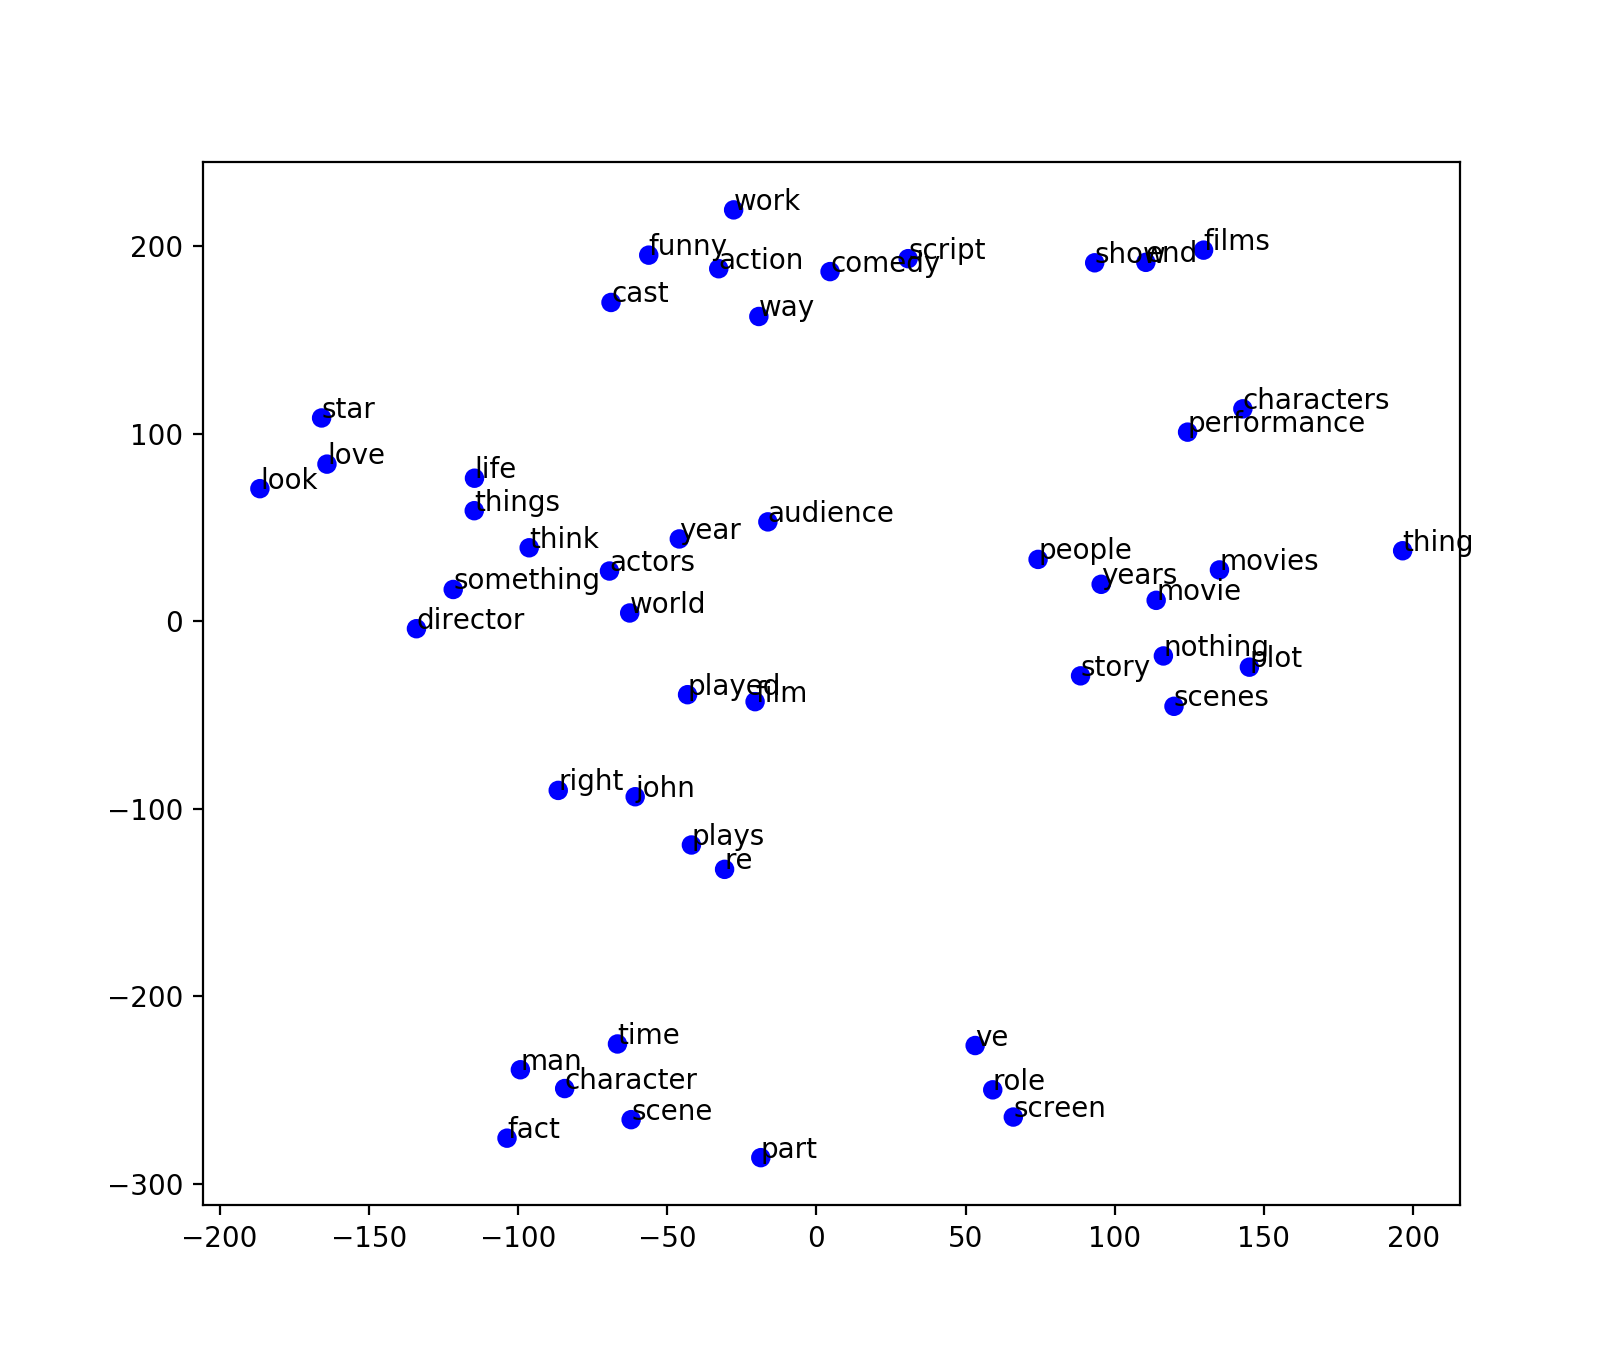
\includegraphics[width=1\textwidth]{figs/nouns.png}
       \caption{Two-dimensional t-SNE projection of doc2vec embeddings of the 50 most frequent nouns}
       \label{figure:nouns}
    \end{minipage}\hfill
    \begin{minipage}{0.49\textwidth}
       \centering
       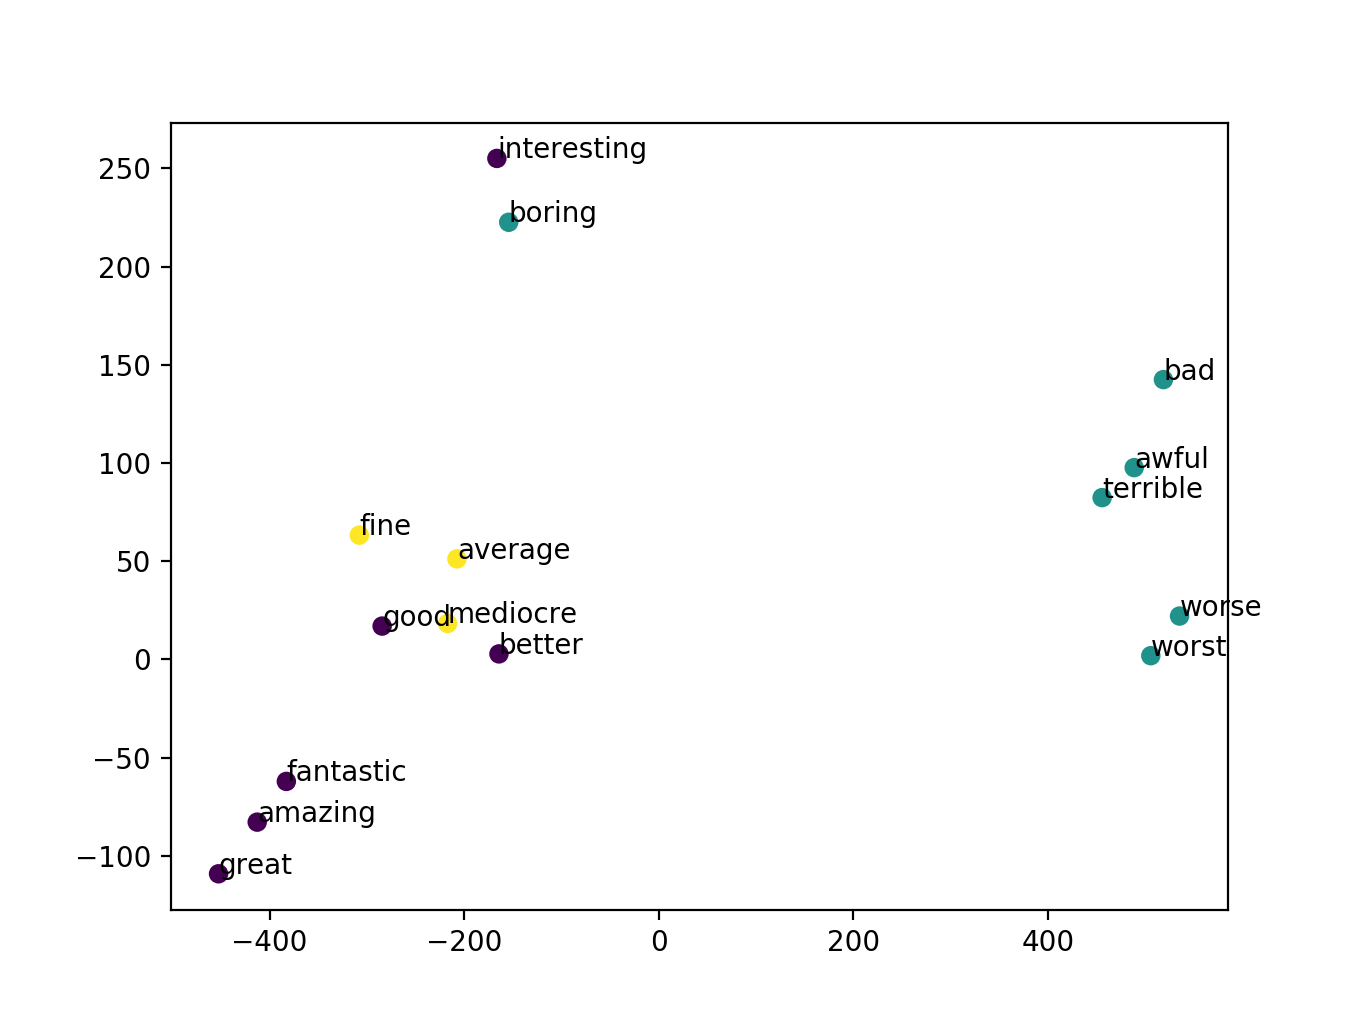
\includegraphics[width=1\textwidth]{figs/sentiment.png}
       \caption{Two-dimensional t-SNE projection of doc2vec adjective embeddings}
       \label{figure:sentiments}
    \end{minipage}
\end{figure*}

\section{Discussion}

My results show that the more complicated \docvec~model, considering the \emph{context} of words, performs better at sentiment analysis than the simple bag-of-word models for generating document vectors. Using T-sne and heatmap graphs, I can qualitatively examine what the model is doing.

Plotting the 50 most frequent nouns in our 2000 files using t-SNE reveals how \docvec~learns contex, seen in Figure \ref{figure:nouns}. Nouns used in the same context such as \emph{plot, story} and \emph{man, character} are grouped together and are thus represented by similar vectors in the \docvec~embedded vector space.

I hypothesise that \docvec~learns sentiments of common adjectives from their usage in the positive and negative files that \docvec~is trained on. I plotted these adjectives using t-SNE in Figure~\ref{figure:sentiments}.

\begin{tablehere}
\centering
 \begin{tabular}{| c | c | c|}  
 \hline
Word & Positive & Negative \\ [0.5ex] 
 \hline\hline
 amazing & 2004 & 516 \\
 \hline
 good & 15025 & 14728 \\ 
 \hline
bad & 3747 & 14726 \\
 \hline
average & 595 & 831 \\
 \hline
\end{tabular}
\caption{Occurrences of words in positive and negative training files} \label{table:occurrences}
\end{tablehere}

I observe that the model seems to learn the sentiment of these adjectives. \emph{Fantastic, amazing, great} are grouped together and \emph{bad, awful, terrible, worse, worst} are also grouped. Interestingly, the neutral adjectives \emph{fine, average, mediocre} seem to be grouped with the positive adjectives \emph{good, better}. This may be due to the comparative occurrence of these adjectives in positive and negative files. As seen in Table \ref{table:occurrences}, the words \emph{amazing} and \emph{bad} dominate in positive and negative files respectively whereas the words \emph{good} and \emph{average} are distributed more evenly between positive and negative files.

\citet{li2015visualizing} proposed a method to visualise indicator words by plotting the variance of word vectors in a sentence against each other. Figure \ref{figure:goodbad} shows a variance visualisation of the sentence \emph{``this has to be one of the greatest movies of all time''}; each grid corresponds to $ ||e_{i,j} - \frac{1}{N_{s}} \sum_{i'\in N_{s}}e_{i',j} ||^{2} $ where $e_{i,j}$ denotes the value for $j$th dimension of word $i$ and $N$ denotes the number of token within the sentences. This gives the word \emph{greatest} as the strongest indicator for this sentence.

A heat-map visualisation of three short reviews, shown in Figure \ref{figure:goodbad}, reveals another analysis that \docvec~learns sentiment; the neutral review seems to lie between the heat-maps of the positive and negative reviews.

\begin{figure*}[t]
    \centering
    \begin{minipage}{0.49\textwidth}
       \centering
       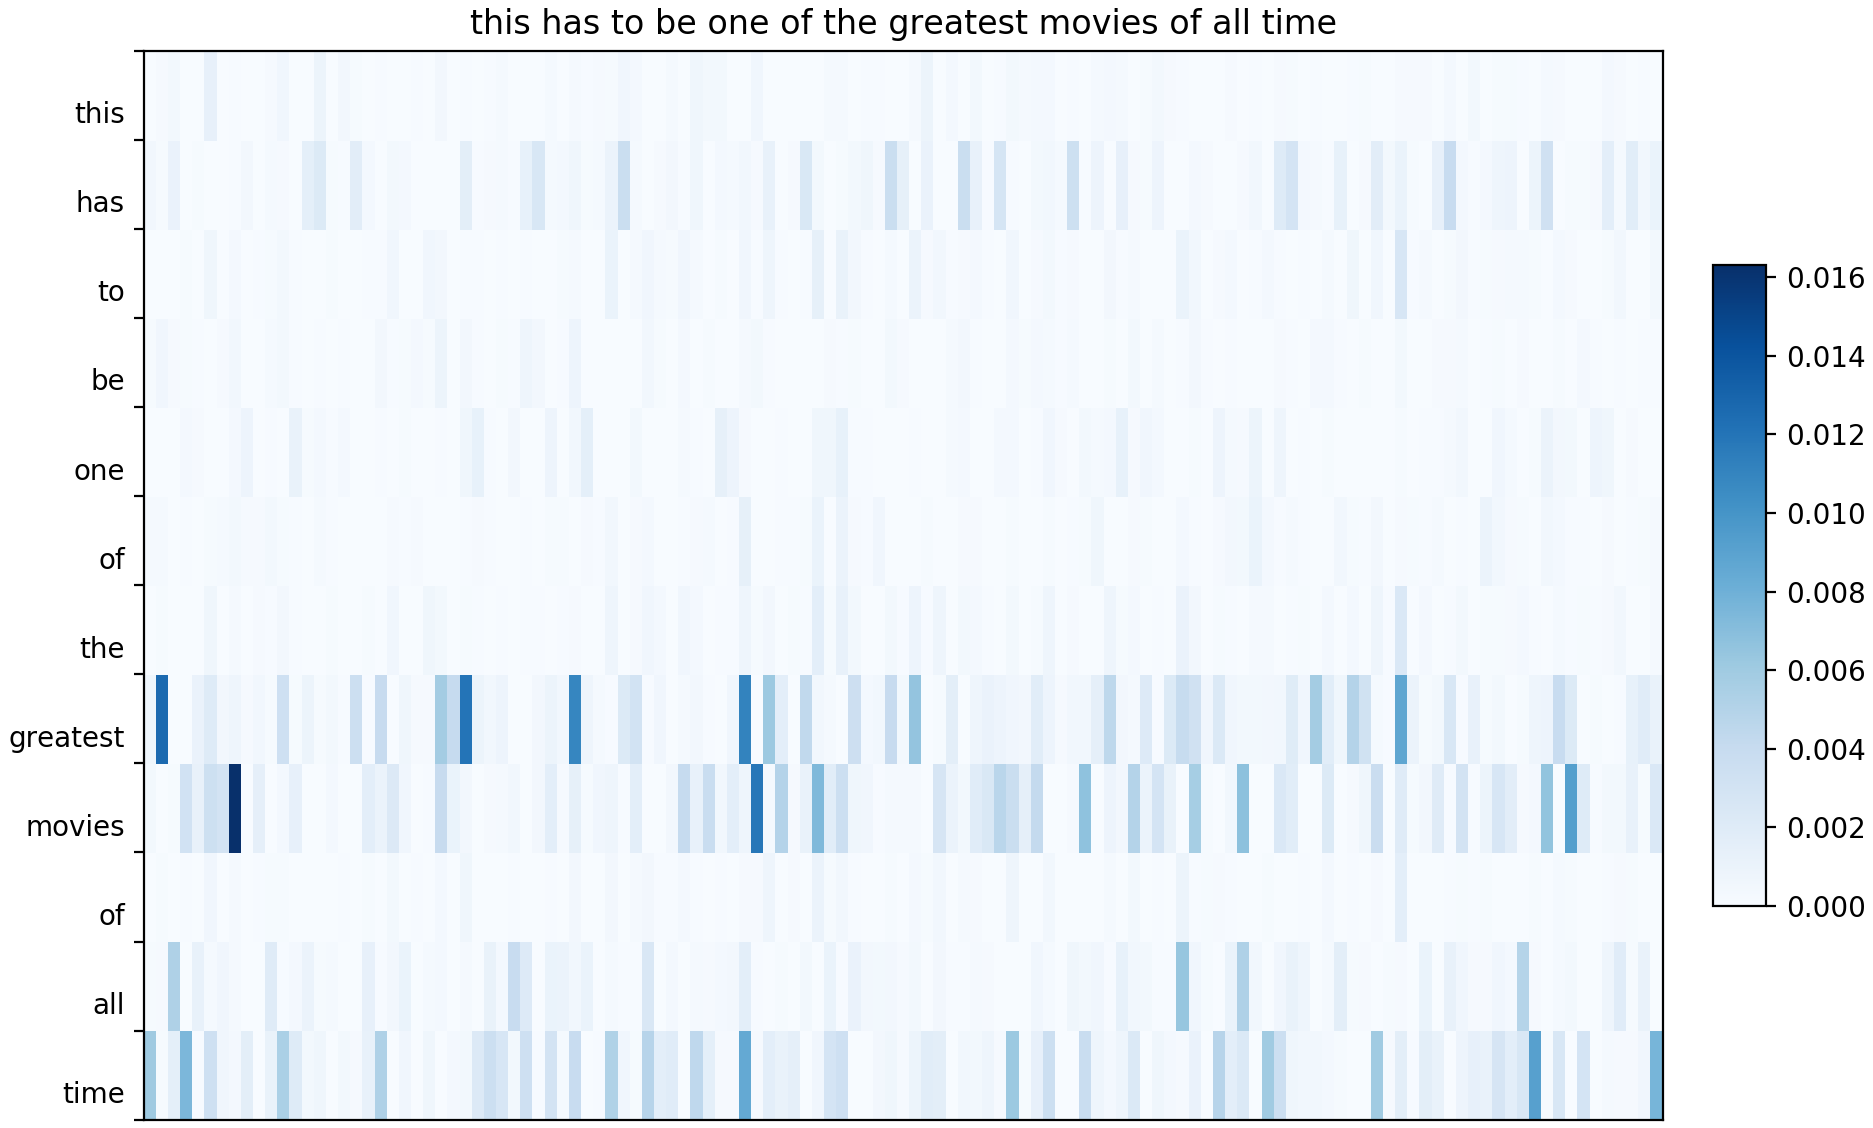
\includegraphics[width=1\textwidth]{figs/greatest.png}
       \caption{Variance visualisation of a single-sentence review}
       \label{figure:greatest}
    \end{minipage}\hfill
    \begin{minipage}{0.49\textwidth}
       \centering
       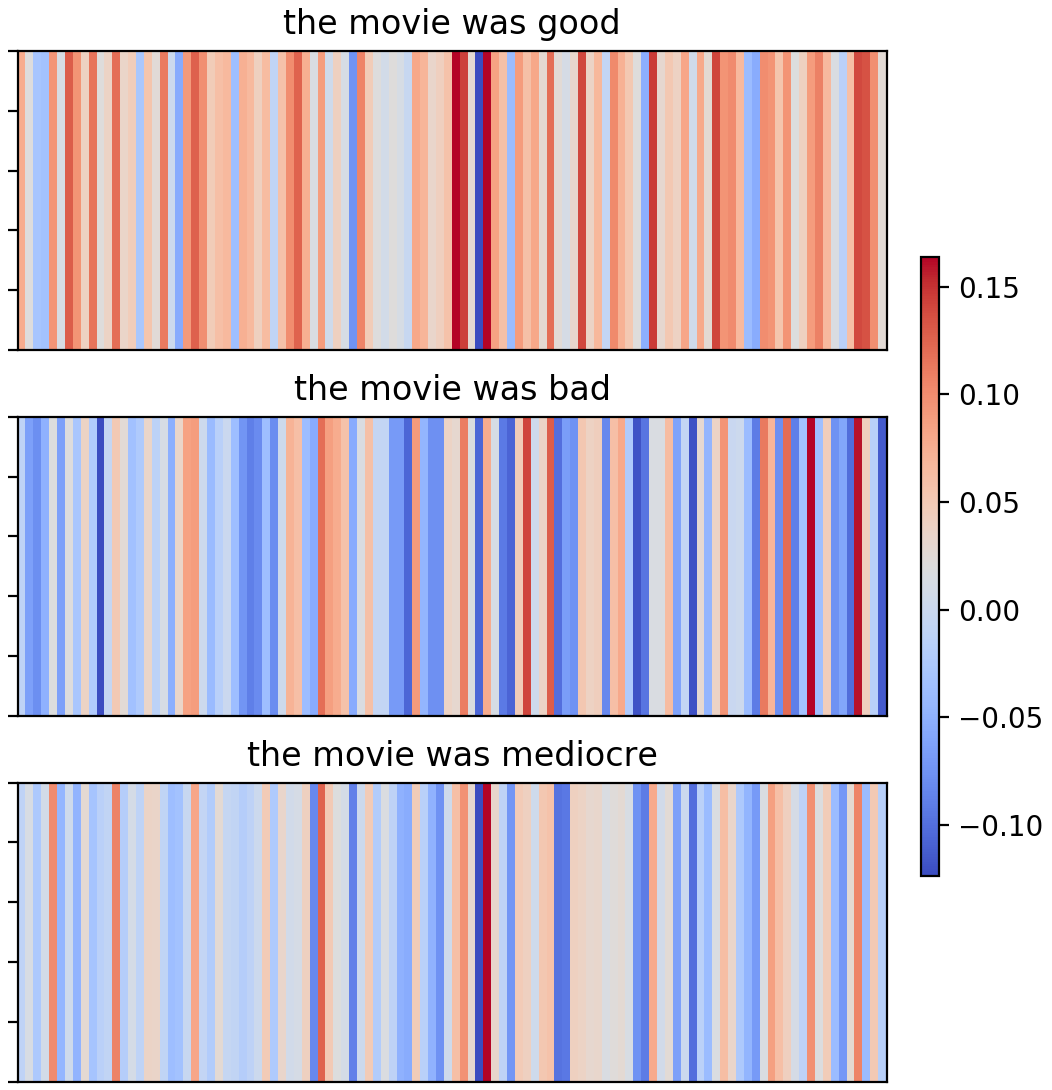
\includegraphics[width=1\textwidth]{figs/goodbad.png}
       \caption{Heat-map visualisation of a good, bad and neutral sentiments}
       \label{figure:goodbad}
    \end{minipage}
\end{figure*}

\section*{Conclusion}

I have shown how using \docvec~vectors in an SVM classifier outperforms naive frequency-based vectors and presence-based vectors. I further qualitatively analysed the behaviour of \docvec, finding that the model learns sentiment through occurrence of adjectives in positive and negative documents.

\bibliography{refs}
\bibliographystyle{apalike}

\end{multicols}
\end{document}